\documentclass[
11pt, % The default document font size, options: 10pt, 11pt, 12pt
%codirector, % Uncomment to add a codirector to the title page
]{charter} 




% El títulos de la memoria, se usa en la carátula y se puede usar el cualquier lugar del documento con el comando \ttitle
\titulo{Sistema de filtrado de agua para laboratorios} 

% Nombre del posgrado, se usa en la carátula y se puede usar el cualquier lugar del documento con el comando \degreename
\posgrado{Carrera de Especialización en Sistemas Embebidos} 
%\posgrado{Carrera de Especialización en Internet de las Cosas} 
%\posgrado{Carrera de Especialización en Intelegencia Artificial}
%\posgrado{Maestría en Sistemas Embebidos} 
%\posgrado{Maestría en Internet de las cosas}

% Tu nombre, se puede usar el cualquier lugar del documento con el comando \authorname
\autor{Ing. Agustín Miguel Grosso} 

% El nombre del director y co-director, se puede usar el cualquier lugar del documento con el comando \supname y \cosupname y \pertesupname y \pertecosupname
\director{Ing. Juan Antonio Tántera}
\pertenenciaDirector{UTN FRBA. Galileo Technologies S.A.} 
% FIXME:NO IMPLEMENTADO EL CODIRECTOR ni su pertenencia
\codirector{} % para que aparezca en la portada se debe descomentar la opción codirector en el documentclass
\pertenenciaCoDirector{}

% Nombre del cliente, quien va a aprobar los resultados del proyecto, se puede usar con el comando \clientename y \empclientename
\cliente{Marcelo Ricci}
\empresaCliente{Ingeniería Clínica}

% Nombre y pertenencia de los jurados, se pueden usar el cualquier lugar del documento con el comando \jurunoname, \jurdosname y \jurtresname y \perteunoname, \pertedosname y \pertetresname.
\juradoUno{Nombre y Apellido (1)}
\pertenenciaJurUno{pertenencia (1)} 
\juradoDos{Nombre y Apellido (2)}
\pertenenciaJurDos{pertenencia (2)}
\juradoTres{Nombre y Apellido (3)}
\pertenenciaJurTres{pertenencia (3)}
 
\fechaINICIO{20 de octubre de 2022}		%Fecha de inicio de la cursada de GdP \fechaInicioName
\fechaFINALPlan{8 de diciembre de 2022} 	%Fecha de final de cursada de GdP
\fechaFINALTrabajo{a confirmar}	%Fecha de defensa pública del trabajo final


\begin{document}

\maketitle
\thispagestyle{empty}
\pagebreak


\thispagestyle{empty}
{\setlength{\parskip}{0pt}
\tableofcontents{}
}
\pagebreak


\section*{Registros de cambios}
\label{sec:registro}


\begin{table}[ht]
\label{tab:registro}
\centering
\begin{tabularx}{\linewidth}{@{}|c|X|c|@{}}
\hline
\rowcolor[HTML]{C0C0C0} 
Revisión & \multicolumn{1}{c|}{\cellcolor[HTML]{C0C0C0}Detalles de los cambios realizados} & Fecha      \\ \hline
0      & Creación del documento                                 &\fechaInicioName \\ \hline
1      & Redacción del acta de constitución del proyecto \newline
		 Identificación y análisis de los interesados \newline
		 Redacción de la descripción técnica-conceptual \newline
		 Definición del propósito y alcance del proyecto & 2 de noviembre de 2022 \\ \hline
2      & Definición de los requerimientos \newline
		 Definición de las historias de usuario (\textit{Product backlog}) \newline
		 Declaración de los entregables del proyecto  \newline
		 Desglose de tareas & 11 de noviembre de 2022 \\ \hline
%3      & Se completa hasta el punto 11 inclusive                & dd/mm/aaaa \\ \hline
%4      & Se completa el plan	                                 & dd/mm/aaaa \\ \hline
\end{tabularx}
\end{table}

\pagebreak



\section*{Acta de constitución del proyecto}
\label{sec:acta}

\begin{flushright}
Buenos Aires, \fechaInicioName
\end{flushright}

\vspace{2cm}

Por medio de la presente se acuerda con el \authorname\hspace{1px} que su Trabajo Final de la \degreename\hspace{1px} se titulará ``\ttitle'', consistirá esencialmente en el desarrollo de un equipo capaz de proveer agua con características adecuadas para análisis médicos, y tendrá un presupuesto preliminar estimado de 600 hs de trabajo, con fecha de inicio \fechaInicioName\hspace{1px} y fecha de presentación pública \fechaFinalName.

Se adjunta a esta acta la planificación inicial.

\vfill

% Esta parte se construye sola con la información que hayan cargado en el preámbulo del documento y no debe modificarla
\begin{table}[ht]
\centering
\begin{tabular}{ccc}
\begin{tabular}[c]{@{}c@{}}Ariel Lutenberg \\ Director posgrado FIUBA\end{tabular} & \hspace{2cm} & \begin{tabular}[c]{@{}c@{}}\clientename \\ \empclientename \end{tabular} \vspace{2.5cm} \\ 
\multicolumn{3}{c}{\begin{tabular}[c]{@{}c@{}} \supname \\ Director del Trabajo Final\end{tabular}} \vspace{2.5cm} \\
%\begin{tabular}[c]{@{}c@{}}\jurunoname \\ Jurado del Trabajo Final\end{tabular}     &  & \begin{tabular}[c]{@{}c@{}}\jurdosname\\ Jurado del Trabajo Final\end{tabular}  \vspace{2.5cm}  \\
%\multicolumn{3}{c}{\begin{tabular}[c]{@{}c@{}} \jurtresname\\ Jurado del Trabajo Final\end{tabular}} \vspace{.5cm}                                                                     
\end{tabular}
\end{table}


\pagebreak

\section{1. Descripción técnica-conceptual del proyecto a realizar}
\label{sec:descripcion}

Aquellas tareas que deben ser realizadas en ambientes protegidos de la contaminación natural como lo son las salas limpias y los laboratorios, deben tener garantizado un estado continuo y controlado de muchos parámetros clave ambientales y de procesos. En las tareas de bioquímica, más específicamente el análisis de muestras de sangre, es necesaria la garantía de provisión continua de agua tipo I y/o II cuyas características se detallan en el cuadro \ref{tab:aguaTipoII}.

\begin{table}[ht]
\begin{tabularx}{\linewidth}{@{}|l|X|X|X|l|@{}}
\hline
\rowcolor[HTML]{C0C0C0}
Parámetro          												&Tipo I 	&Tipo II 	&Tipo III  	&Tipo IV 	\\ \hline
Conductividad eléctrica máx. [$\mu$S/cm @ 25 \textcelsius)    	&0,056 		&1,0 		&4,0 		&5,0		\\ \hline
Resistividad eléctrica mín. (M$\Omega$ cm @ 25 \textcelsius)	&18,2 		&1,0		&0,25 		&0,2		\\ \hline
PH a 25 \textcelsius											&-			&- 			&-			&5,0 - 8,0	\\ \hline
TOC máx. ($\mu$g/l)												&10			&50 		&200		&Sin límite	\\ \hline
Sodio máx. ($\mu$g/l)											&1			&5 			&10			&50			\\ \hline
Sílice máx. ($\mu$g/l)											&3			&3 			&500		&Sin límite	\\ \hline
Cloro máx. ($\mu$g/l)											&1			&5 			&10			&50			\\ \hline
\end{tabularx}

\caption{\centering Especificaciones sobre los tipos de agua según ASTM D1193-91 (\textit{American Society for Testing and Materials}).}
\label{tab:aguaTipoII}
\end{table}

Los equipos analizados disponibles en el mercado son dispositivos que contienen módulos para filtrado (carbón activado, filtros de partículas, cartuchos de ósmosis inversa) de gran tamaño para garantizar una vida útil funcional aceptable antes del reemplazo recomendado. También, ciertos parámetros que pueden verse alterados por la finalización del correcto funcionamiento de dichos módulos, en muchos casos, deben ser monitoreados y medidos de forma manual con cierta regularidad para detectar la necesidad de mantenimiento y/o cambio.

El actual desarrollo, además de cumplir con la pauta principal que es la erogación del agua definida, incorporará el control continuo del estado del sistema:
\begin{itemize}
	\item Control de vida útil de módulos.
	\item Protección del sistema mediante medición de presiones.
	\item Detección e informe de fallas de cada etapa.
	\item Resguardo de información para análisis posteriores.
\end{itemize}

La principal ventaja de un control continuo y reportado es la posibilidad de realizar mantenimientos preventivos. La disponibilidad de información sobre el estado del sistema permite evitar que ciertos desvíos decanten en fallas críticas. 
También, las alertas sobre la vida útil de los distintos módulos de filtrado permiten adelantarse al recambio de estos módulos y vuelve más eficiente el esquema de mantenimiento. Este esquema de análisis y reportes posibilita el uso de módulos menor tamaño y, por lo tanto, el equipo se vuelve más pequeño y cómodo para ser manipulado.


Como segunda parte del proyecto (no incluida en este plan) se encuentra el objetivo de incorporar los equipos a una red de IoT (\textit{Internet of Things}) para el monitoreo del universo de equipos por parte del proveedor y permitiéndole elaborar esquemas de servicio técnico preventivo.

Se muestra, a continuación, un diagrama en bloques de la solución propuesta:

\begin{figure}[htpb]
\centering 
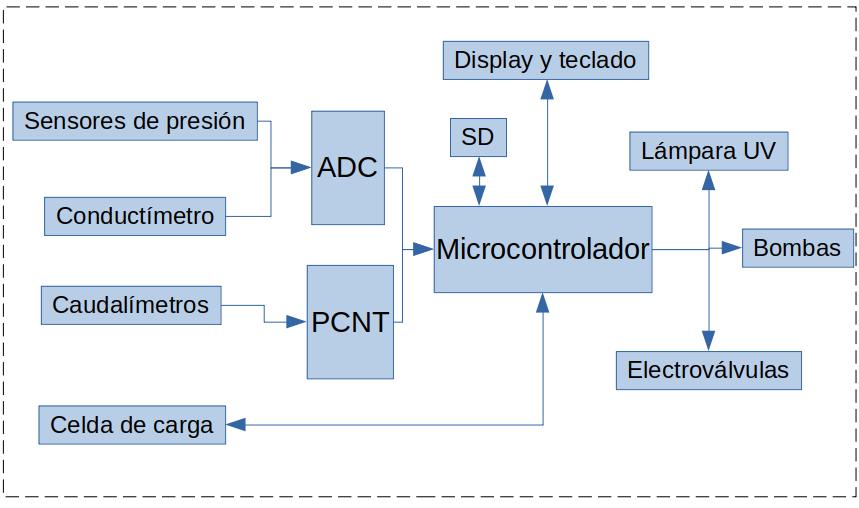
\includegraphics[width=.7\textwidth]{./Figuras/Microcontrolador y sus perifericos.png}
\caption{Microcontrolador y sus periféricos.}
\label{fig:microcontroladorConexiones}
\end{figure}

\vspace{25px}

El núcleo lógico del sistema será un módulo ESP32 con FreeRTOS (\textit{Free Real Time Operating System}) como sistema operativo. El microcontrolador será el encargado de leer las diferentes variables, analizarlas y actuar, como así también, deberá realizar tareas de almacenamiento de información y de comunicación con el usuario (teclado y display).
Mediante la lectura de periféricos se analizarán variables para diferentes funciones:
\begin{itemize}
	\item Presión
	\begin{itemize}
		\item Detección de obstrucciones.
		\item Detección de fluido a la entrada.
		\item Análisis del estado de filtros.
	\end{itemize}
	\item Caudal	
	\begin{itemize}
		\item Detección de obstrucciones.
		\item Medición de agua erogada.
		\item Análisis del estado de filtros.
	\end{itemize}
	\item Conductividad
	\begin{itemize}
		\item Medición de estado del agua filtrada.
	\end{itemize}
	\item Peso
	\begin{itemize}
		\item Medición del estado de llenado del reservorio.
	\end{itemize}
\end{itemize}

Los salidas del sistema sobre los cuales se actuará serán bombas, electro-válvulas y una lámpara UV (eliminación de agentes biológicos) para diferentes etapas:
\begin{itemize}
	\item Ingreso de agua al equipo.
	\item Eliminación del descarte de las ósmosis.
	\item Llenado de reservorio.
	\item Re-circulación para el filtrado.
	\item Erogación de agua.
\end{itemize}


\vspace{25px}
\begin{figure}[htpb]
\centering 
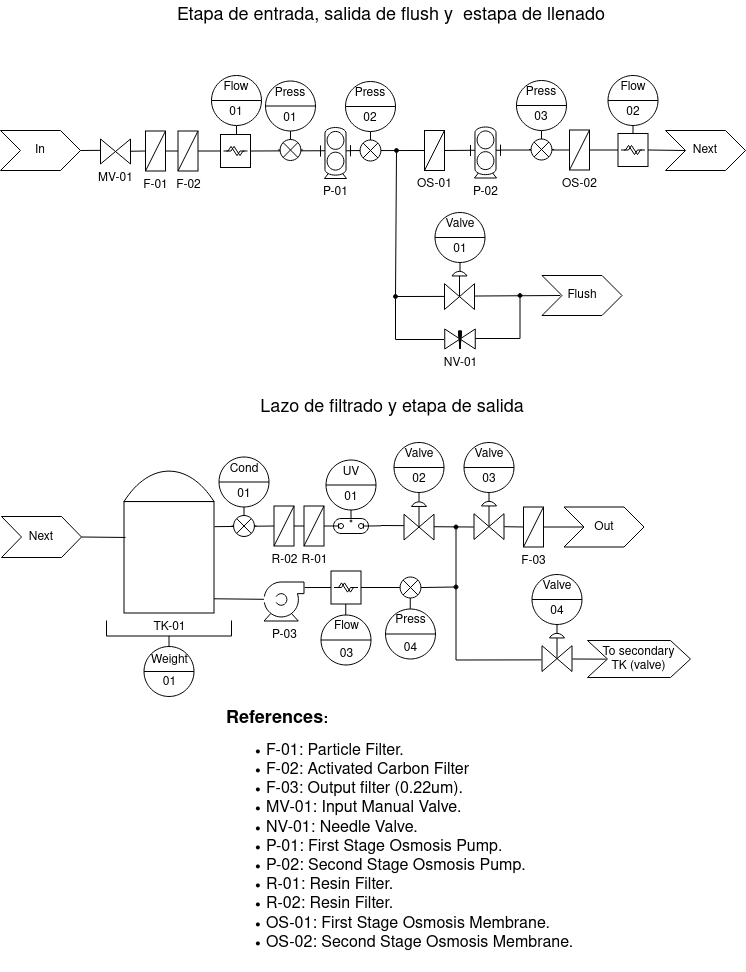
\includegraphics[width=.8\textwidth]{./Figuras/Esquema de equipo_vert.png}
\caption{Esquema del equipo de filtrado.}
\label{fig:equipoEsquemaFisico}
\end{figure}

\vspace{25px}
\newpage
\section{2. Identificación y análisis de los interesados}
\label{sec:interesados}

\begin{table}[ht]
%\caption{Identificación de los interesados}
%\label{tab:interesados}
\begin{tabularx}{\linewidth}{@{}|l|X|X|l|@{}}
\hline
\rowcolor[HTML]{C0C0C0} 
Rol           & Nombre y Apellido 		& Organización 		& Puesto 			\\ \hline
Cliente       & \clientename 			&\empclientename 	& Gerente 			\\ \hline
Responsable   & \authorname 			& FIUBA        		& Alumno 			\\ \hline
Orientador    & \supname 				& \pertesupname 	& Director 			\\ \hline
Equipo        & José Alejandro Tántera 	& GA.MA ITALY 		& Desarrollador de hardware    	\\ \hline
Usuario final & Laboratorios de análisis clínicos           &       -       	&      -  	\\ \hline
\end{tabularx}
\end{table}

\section{3. Propósito del proyecto}
\label{sec:proposito}

El propósito de este proyecto es garantizar la provisión de agua filtrada a laboratorios de análisis clínicos para, principalmente, la tarea de disolución de sangre. El sistema deberá ser capaz de suministrar agua a usuarios, mediante la solicitud a través de la interfaz correspondiente, y a un segundo sistema que se encontrará conectado a una salida dedicada.

A su vez, tiene el propósito de ser el primer proyecto del equipo de desarrollos electrónicos que se formará entre las personas que aquí participan como director, colaborador y alumno.

\section{4. Alcance del proyecto}
\label{sec:alcance}

Se encuentra dentro del alcance del proyecto el desarrollo del firmware que implementará la lógica del sistema, el sensado de variables externas y la actuación sobre los dispositivos de salida. Como así también el prototipo de hardware del sistema embebido. 
El sistema embebido resultante del presente desarrollo será incorporado al equipo para realizar las pruebas de campo junto a las conexiones, los filtros, el reservorio, etc.

No se encuentra comprendido dentro del alcance del trabajo el diseño y la construcción de la estructura del equipo, el conexionado entre cada elemento y la selección de los filtros de partículas, lámpara UV y demás dispositivos externos.
El proyecto no incluye pruebas ni habilitaciones en institutos o entes de regulación.


\section{5. Supuestos del proyecto}
\label{sec:supuestos}

Para el desarrollo en tiempo y forma del presente proyecto se supone que:
\begin{itemize}
	\item El cliente no interrumpirá el proyecto.
	\item Todos los módulos que comprenden el proyecto pueden ser adquiridos.
	\begin{itemize}
		\item Microcontrolador ESP32.
		\item Expansor de GPIO (MCP23008 o MCP23017).
		\item Celda de carga y módulo HX711.
	\end{itemize}
	\item La fabricación del hardware no se verá demorada por factores externos al proyecto y al equipo de desarrollo.
	\item Los desarrolladores (alumno y colaborador) cuentan con la disponibilidad de 12 horas por semana.
	\item Se cuenta con la documentación necesaria sobre los dispositivos utilizados.
	\item La estructura y el conexionado del equipo estarán listos para realizar la prueba de campo.
\end{itemize}

\section{6. Requerimientos}
\label{sec:requerimientos}

\begin{enumerate}
	\item Requerimientos funcionales
		\begin{enumerate}
			\item Deben garantizarse las propiedades de agua tipo II a la salida.
			\item El usuario debe poder solicitar la erogación.
			\item El sistema debe proveer agua a un segundo equipo automáticamente.
			\item Debe detectarse cuándo el segundo equipo debe ser provisto.
			\item El ingreso de agua al sistema, el llenado del reservorio y el filtrado deben ser automáticos.
			\item Deben ser detectadas obstrucciones en filtros.
			\item Debe analizarse la vida útil de los filtros.
			\item Debe almacenarse información para posteriores análisis.
		\end{enumerate}
	\item Requerimientos de metodología de trabajo
		\begin{enumerate}
			\item Control de versiones mediante GIT.
			\item Aplicación de reglas de programación MISRA C.
			\item Esquemáticos del hardware desarrollados en Altium.
		\end{enumerate}
\end{enumerate}

\section{7. Historias de usuarios (\textit{Product backlog})}
\label{sec:backlog}

\begin{itemize}
\item Historia de usuario 1
\\El usuario requiere de un sistema que utilice la red de agua corriente como fuente de alimentación.
	\begin{itemize}
		\item Dificultad: baja (1)
		\\Implica el análisis de la presión a la entrada del equipo.
		\item Complejidad: baja (1)
		\\Análisis de un solo sensor de presión.
		\item Riesgo: medio (3)
		\\Sin un correcto funcionamiento el sistema se desabastece.
	\end{itemize}
\textit{Story point:} 5
\item Historia de usuario 2
\\El usuario requiere de la disponibilidad constante de agua mediante un reservorio con contenido controlado.
	\begin{itemize}
		\item Dificultad: media (3)
		\\Implica el análisis de sensores de presión, caudalímetros y celdas de carga. También, se debe gestionar la activación de bombas y electro-válvulas.
		\item Complejidad: media (3)
		\\La lógica debe analizar y comandar los periféricos para abastecer y mantener el contenido del tanque.
		\item Riesgo: medio (3)
		\\Sin un correcto funcionamiento el sistema se desabastece o el reservorio podría desbordarse.
	\end{itemize}
\textit{Story point:} 9
\item  Historia de usuario 3
\\El usuario debe disponer de agua tipo II (ver tabla \ref{tab:aguaTipoII}).
	\begin{itemize}
		\item Dificultad: alta (5)
		\\Medición de variables clave. 
		\item Complejidad: : media (3)
		\\Control del lazo de filtrado.
		\item Riesgo: alto (5)
		\\Es el bloque que debe garantizar la calidad del agua filtrada. Afecta a los procesos que requieren de agua tipo II.
	\end{itemize}
\textit{Story point:} 13
\item  Historia de usuario 4
\\El usuario requiere la posibilidad de obtener agua a demanda.
	\begin{itemize}
		\item Dificultad: : media (3)
		\\Dispensación de agua y control del caudal.
		\item Complejidad: media (3)
		\\Control del lazo de erogación y medición del agua erogada.
		\item Riesgo: bajo (1)
		\\El usuario puede corregir algún error en la cantidad de agua entregada.
	\end{itemize}
\textit{Story point:} 7
\item  Historia de usuario 5
\\El usuario precisa que un segundo equipo sea provisto de agua por el sistema.
	\begin{itemize}
		\item Dificultad: baja (1)
		\\Dispensación de agua sin control exacto de caudal.
		\item Complejidad: media (3)
		\\Detección de necesidad de erogación a través de una rutina de medición de caudal. Fin del proceso cuando el segundo sistema cierre su válvula de entrada.
		\item Riesgo: alto (5)
		\\El equipo provisto de agua puede quedar desabastecido y afectar los procesos dependientes de este.
	\end{itemize}
\textit{Story point:} 9
\end{itemize}

\section{8. Entregables principales del proyecto}
\label{sec:entregables}

Los entregables del proyecto son:

\begin{itemize}
	\item Manual de uso
	\item Firmware
	\item Diagrama de circuitos esquemáticos
	\item Informe final
\end{itemize}

\section{9. Desglose del trabajo en tareas}
\label{sec:wbs}

\begin{enumerate}
\item Gestión del Proyecto 
	\begin{enumerate}	
	\item Definición de los requerimientos en conjunto con el cliente (8 h)
	\item Definición inicial de la solución de hardware y software (16 h)
	\item Planeamiento inicial (8 h)
	\item Presentación de la propuesta al cliente (6 h)
	\item Ajustes de requerimientos (8 h)
	\item Documentación del alcance y planeamiento del proyecto. (24 h)
	\end{enumerate}
\item Investigación
	\begin{enumerate}
	\item Periféricos (32 h)
		\begin{itemize}
			\item Celda de carga
			\item Caudalímetro
			\item Sensor de presión
			\item Conductímetro
			\item Memoria SD
			\item Display
		\end{itemize}
	\item Microcontrolador (16 h)
	\item Componentes adicionales (32 h)
		\begin{itemize}
			\item Expansor de GPIO
			\item Transistores
			\item Driver para transistores
			\item Otros
		\end{itemize}
	\item Fabricantes (4 h)
	\end{enumerate}
\item Desarrollo de hardware
	\begin{enumerate}
	\item Diseño de diagramas esquemáticos (40 h)
	\item Diseño de PCB (32 h)
	\end{enumerate}
\item Desarrollo de software
	\begin{enumerate}
	\item \textit{Device Drivers}
		\begin{itemize}
			\item Celda de carga HX711 (16 h)
			\item Bomba (6 h)
			\item Electro-válvula (4 h)
			\item Lámpara UV (4 h)
			\item Caudalímetro (16 h)
			\item Sensor de presión (8 h)
			\item Conductímetro (8 h)
			\item Módulo SD (16 h)
			\item Display (32 h)
			\item Teclado (16 h)
		\end{itemize}
	\item Diseño de la MEF (Máquina de Estados Finitos) (8 h)
	\item Programación de tareas de \textit{FreeRTOS} (24 h)
	\item Programación de la MEF (24 h)
	\end{enumerate}
\item Prueba y verificación
	\begin{enumerate}
		\item Planificación (16 h)
		\item \textit{Device Drivers} (24 h)
		\item Lógica del sistema (8 h)
		\item Sistema integrado (40 h)
		\item Modificaciones (40 h)
	\end{enumerate}
\item Documentación
	\begin{enumerate}
		\item Elaboración del manual de uso (24 h)
		\item Elaboración del informe final (60 h)
	\end{enumerate}
\end{enumerate}

Cantidad total de horas: 620 h.

\section{10. Diagrama de Activity On Node}
\label{sec:AoN}

\begin{consigna}{red}
Armar el AoN a partir del WBS definido en la etapa anterior. 

%La figura \ref{fig:AoN} fue elaborada con el paquete latex tikz y pueden consultar la siguiente referencia \textit{online}:

%\url{https://www.overleaf.com/learn/latex/LaTeX_Graphics_using_TikZ:_A_Tutorial_for_Beginners_(Part_3)\%E2\%80\%94Creating_Flowcharts}

\end{consigna}

\begin{figure}[htpb]
\centering 
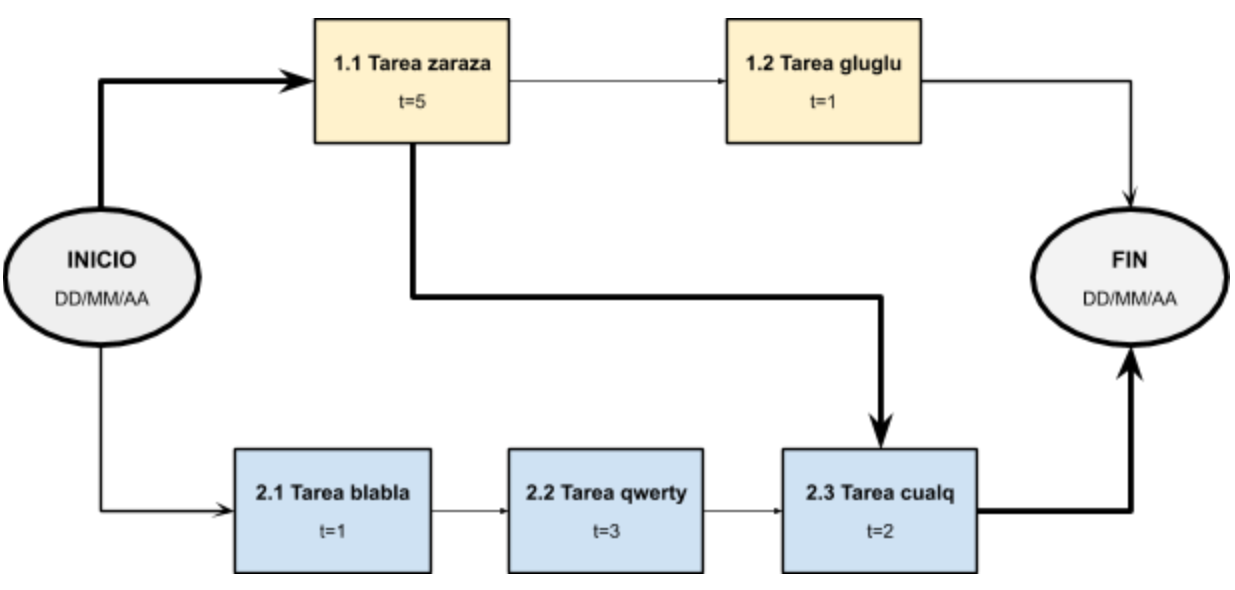
\includegraphics[width=.8\textwidth]{./Figuras/AoN.png}
\caption{Diagrama en \textit{Activity on Node}}
\label{fig:AoN}
\end{figure}

Indicar claramente en qué unidades están expresados los tiempos.
De ser necesario indicar los caminos semicríticos y analizar sus tiempos mediante un cuadro.
Es recomendable usar colores y un cuadro indicativo describiendo qué representa cada color, como se muestra en el siguiente ejemplo:



\section{11. Diagrama de Gantt}
\label{sec:gantt}

\begin{consigna}{red}

Existen muchos programas y recursos \textit{online} para hacer diagramas de gantt, entre los cuales destacamos:

\begin{itemize}
\item Planner
\item GanttProject
\item Trello + \textit{plugins}. En el siguiente link hay un tutorial oficial: \\ \url{https://blog.trello.com/es/diagrama-de-gantt-de-un-proyecto}
\item Creately, herramienta online colaborativa. \\\url{https://creately.com/diagram/example/ieb3p3ml/LaTeX}
\item Se puede hacer en latex con el paquete \textit{pgfgantt}\\ \url{http://ctan.dcc.uchile.cl/graphics/pgf/contrib/pgfgantt/pgfgantt.pdf}
\end{itemize}

Pegar acá una captura de pantalla del diagrama de Gantt, cuidando que la letra sea suficientemente grande como para ser legible. 
Si el diagrama queda demasiado ancho, se puede pegar primero la ``tabla'' del Gantt y luego pegar la parte del diagrama de barras del diagrama de Gantt.

Configurar el software para que en la parte de la tabla muestre los códigos del EDT (WBS).\\
Configurar el software para que al lado de cada barra muestre el nombre de cada tarea.\\
Revisar que la fecha de finalización coincida con lo indicado en el Acta Constitutiva.

En la figura \ref{fig:gantt}, se muestra un ejemplo de diagrama de gantt realizado con el paquete de \textit{pgfgantt}. En la plantilla pueden ver el código que lo genera y usarlo de base para construir el propio.

\begin{figure}[htbp]
\begin{center}
\begin{ganttchart}{1}{12}
  \gantttitle{2020}{12} \\
  \gantttitlelist{1,...,12}{1} \\
  \ganttgroup{Group 1}{1}{7} \\
  \ganttbar{Task 1}{1}{2} \\
  \ganttlinkedbar{Task 2}{3}{7} \ganttnewline
  \ganttmilestone{Milestone o hito}{7} \ganttnewline
  \ganttbar{Final Task}{8}{12}
  \ganttlink{elem2}{elem3}
  \ganttlink{elem3}{elem4}
\end{ganttchart}
\end{center}
\caption{Diagrama de gantt de ejemplo}
\label{fig:gantt}
\end{figure}


\begin{landscape}
\begin{figure}[htpb]
\centering 
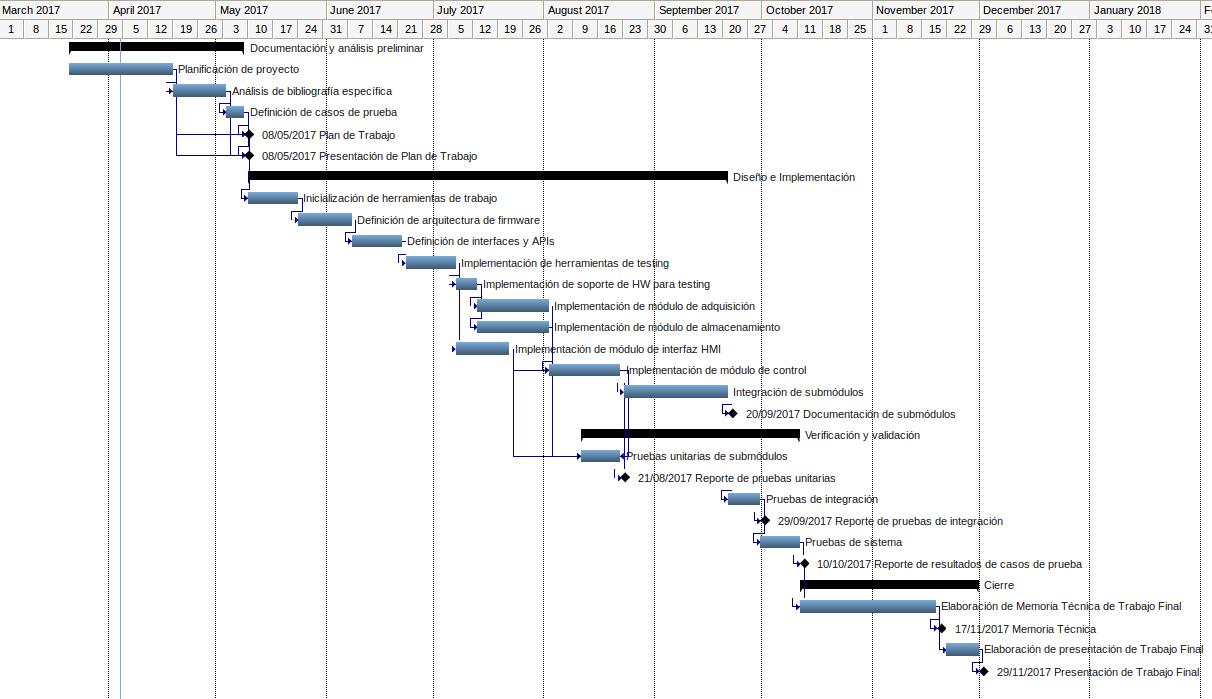
\includegraphics[height=.85\textheight]{./Figuras/Gantt-2.png}
\caption{Ejemplo de diagrama de Gantt rotado}
\label{fig:diagGantt}
\end{figure}

\end{landscape}

\end{consigna}


\section{12. Presupuesto detallado del proyecto}
\label{sec:presupuesto}

\begin{consigna}{red}
Si el proyecto es complejo entonces separarlo en partes:
\begin{itemize}
	\item Un total global, indicando el subtotal acumulado por cada una de las áreas.
	\item El desglose detallado del subtotal de cada una de las áreas.
\end{itemize}

IMPORTANTE: No olvidarse de considerar los COSTOS INDIRECTOS.

\end{consigna}

\begin{table}[htpb]
\centering
\begin{tabularx}{\linewidth}{@{}|X|c|r|r|@{}}
\hline
\rowcolor[HTML]{C0C0C0} 
\multicolumn{4}{|c|}{\cellcolor[HTML]{C0C0C0}COSTOS DIRECTOS} \\ \hline
\rowcolor[HTML]{C0C0C0} 
Descripción &
  \multicolumn{1}{c|}{\cellcolor[HTML]{C0C0C0}Cantidad} &
  \multicolumn{1}{c|}{\cellcolor[HTML]{C0C0C0}Valor unitario} &
  \multicolumn{1}{c|}{\cellcolor[HTML]{C0C0C0}Valor total} \\ \hline
 &
  \multicolumn{1}{c|}{} &
  \multicolumn{1}{c|}{} &
  \multicolumn{1}{c|}{} \\ \hline
 &
  \multicolumn{1}{c|}{} &
  \multicolumn{1}{c|}{} &
  \multicolumn{1}{c|}{} \\ \hline
\multicolumn{1}{|l|}{} &
   &
   &
   \\ \hline
\multicolumn{1}{|l|}{} &
   &
   &
   \\ \hline
\multicolumn{3}{|c|}{SUBTOTAL} &
  \multicolumn{1}{c|}{} \\ \hline
\rowcolor[HTML]{C0C0C0} 
\multicolumn{4}{|c|}{\cellcolor[HTML]{C0C0C0}COSTOS INDIRECTOS} \\ \hline
\rowcolor[HTML]{C0C0C0} 
Descripción &
  \multicolumn{1}{c|}{\cellcolor[HTML]{C0C0C0}Cantidad} &
  \multicolumn{1}{c|}{\cellcolor[HTML]{C0C0C0}Valor unitario} &
  \multicolumn{1}{c|}{\cellcolor[HTML]{C0C0C0}Valor total} \\ \hline
\multicolumn{1}{|l|}{} &
   &
   &
   \\ \hline
\multicolumn{1}{|l|}{} &
   &
   &
   \\ \hline
\multicolumn{1}{|l|}{} &
   &
   &
   \\ \hline
\multicolumn{3}{|c|}{SUBTOTAL} &
  \multicolumn{1}{c|}{} \\ \hline
\rowcolor[HTML]{C0C0C0}
\multicolumn{3}{|c|}{TOTAL} &
   \\ \hline
\end{tabularx}%
\end{table}


\section{13. Gestión de riesgos}
\label{sec:riesgos}

\begin{consigna}{red}
a) Identificación de los riesgos (al menos cinco) y estimación de sus consecuencias:
 
Riesgo 1: detallar el riesgo (riesgo es algo que si ocurre altera los planes previstos de forma negativa)
\begin{itemize}
	\item Severidad (S): mientras más severo, más alto es el número (usar números del 1 al 10).\\
	Justificar el motivo por el cual se asigna determinado número de severidad (S).
	\item Probabilidad de ocurrencia (O): mientras más probable, más alto es el número (usar del 1 al 10).\\
	Justificar el motivo por el cual se asigna determinado número de (O). 
\end{itemize}   

Riesgo 2:
\begin{itemize}
	\item Severidad (S): 
	\item Ocurrencia (O):
\end{itemize}

Riesgo 3:
\begin{itemize}
	\item Severidad (S): 
	\item Ocurrencia (O):
\end{itemize}


b) Tabla de gestión de riesgos:      (El RPN se calcula como RPN=SxO)

\begin{table}[htpb]
\centering
\begin{tabularx}{\linewidth}{@{}|X|c|c|c|c|c|c|@{}}
\hline
\rowcolor[HTML]{C0C0C0} 
Riesgo & S & O & RPN & S* & O* & RPN* \\ \hline
       &   &   &     &    &    &      \\ \hline
       &   &   &     &    &    &      \\ \hline
       &   &   &     &    &    &      \\ \hline
       &   &   &     &    &    &      \\ \hline
       &   &   &     &    &    &      \\ \hline
\end{tabularx}%
\end{table}

Criterio adoptado: 
Se tomarán medidas de mitigación en los riesgos cuyos números de RPN sean mayores a...

Nota: los valores marcados con (*) en la tabla corresponden luego de haber aplicado la mitigación.

c) Plan de mitigación de los riesgos que originalmente excedían el RPN máximo establecido:
 
Riesgo 1: plan de mitigación (si por el RPN fuera necesario elaborar un plan de mitigación).
  Nueva asignación de S y O, con su respectiva justificación:
  - Severidad (S): mientras más severo, más alto es el número (usar números del 1 al 10).
          Justificar el motivo por el cual se asigna determinado número de severidad (S).
  - Probabilidad de ocurrencia (O): mientras más probable, más alto es el número (usar del 1 al 10).
          Justificar el motivo por el cual se asigna determinado número de (O).

Riesgo 2: plan de mitigación (si por el RPN fuera necesario elaborar un plan de mitigación).
 
Riesgo 3: plan de mitigación (si por el RPN fuera necesario elaborar un plan de mitigación).

\end{consigna}


\section{14. Gestión de la calidad}
\label{sec:calidad}

\begin{consigna}{red}
Para cada uno de los requerimientos del proyecto indique:
\begin{itemize} 
\item Req \#1: copiar acá el requerimiento.

\begin{itemize}
	\item Verificación para confirmar si se cumplió con lo requerido antes de mostrar el sistema al cliente. Detallar 
	\item Validación con el cliente para confirmar que está de acuerdo en que se cumplió con lo requerido. Detallar  
\end{itemize}

\end{itemize}

Tener en cuenta que en este contexto se pueden mencionar simulaciones, cálculos, revisión de hojas de datos, consulta con expertos, mediciones, etc.  Las acciones de verificación suelen considerar al entregable como ``caja blanca'', es decir se conoce en profundidad su funcionamiento interno.  En cambio, las acciones de validación suelen considerar al entregable como ``caja negra'', es decir, que no se conocen los detalles de su funcionamiento interno.

\end{consigna}

\section{15. Procesos de cierre}    
\label{sec:cierre}

\begin{consigna}{red}
Establecer las pautas de trabajo para realizar una reunión final de evaluación del proyecto, tal que contemple las siguientes actividades:

\begin{itemize}
	\item Pautas de trabajo que se seguirán para analizar si se respetó el Plan de Proyecto original:
	 - Indicar quién se ocupará de hacer esto y cuál será el procedimiento a aplicar. 
	\item Identificación de las técnicas y procedimientos útiles e inútiles que se emplearon, y los problemas que surgieron y cómo se solucionaron:
	 - Indicar quién se ocupará de hacer esto y cuál será el procedimiento para dejar registro.
	\item Indicar quién organizará el acto de agradecimiento a todos los interesados, y en especial al equipo de trabajo y colaboradores:
	  - Indicar esto y quién financiará los gastos correspondientes.
\end{itemize}

\end{consigna}


\end{document}
